%%%%%%%%%%%%%%%%%%%%%%%%%%%%%%%%%%%%%%%%%
% Beamer Presentation
% LaTeX Template
% Version 1.0 (10/11/12)
%
% This template has been downloaded from:
% http://www.LaTeXTemplates.com
%
% License:
% CC BY-NC-SA 3.0 (http://creativecommons.org/licenses/by-nc-sa/3.0/)
%
%%%%%%%%%%%%%%%%%%%%%%%%%%%%%%%%%%%%%%%%%

%----------------------------------------------------------------------------------------
%	PACKAGES AND THEMES
%----------------------------------------------------------------------------------------

\documentclass{beamer}

\mode<presentation> {
	
	% The Beamer class comes with a number of default slide themes
	% which change the colors and layouts of slides. Below this is a list
	% of all the themes, uncomment each in turn to see what they look like.
	
	%\usetheme{default}
	%\usetheme{AnnArbor}
	%\usetheme{Antibes}
	%\usetheme{Bergen}
	%\usetheme{Berkeley}
	%\usetheme{Berlin}
	%\usetheme{Boadilla}
	%\usetheme{CambridgeUS}
	%\usetheme{Copenhagen}
	%\usetheme{Darmstadt}
	%\usetheme{Dresden}
	%\usetheme{Frankfurt}
	%\usetheme{Goettingen}
	%\usetheme{Hannover}
	%\usetheme{Ilmenau}
	%\usetheme{JuanLesPins}
	%\usetheme{Luebeck}
	\usetheme{Madrid}
	%\usetheme{Malmoe}
	%\usetheme{Marburg}
	%\usetheme{Montpellier}
	%\usetheme{PaloAlto}
	%\usetheme{Pittsburgh}
	%\usetheme{Rochester}
	%\usetheme{Singapore}
	%\usetheme{Szeged}
	%\usetheme{Warsaw}
	
	% As well as themes, the Beamer class has a number of color themes
	% for any slide theme. Uncomment each of these in turn to see how it
	% changes the colors of your current slide theme.
	
	%\usecolortheme{albatross}
	%\usecolortheme{beaver}
	%\usecolortheme{beetle}
	%\usecolortheme{crane}
	%\usecolortheme{dolphin}
	%\usecolortheme{dove}
	%\usecolortheme{fly}
	%\usecolortheme{lily}
	%\usecolortheme{orchid}
	%\usecolortheme{rose}
	%\usecolortheme{seagull}
	%\usecolortheme{seahorse}
	%\usecolortheme{whale}
	%\usecolortheme{wolverine}
	
	%\setbeamertemplate{footline} % To remove the footer line in all slides uncomment this line
	%\setbeamertemplate{footline}[page number] % To replace the footer line in all slides with a simple slide count uncomment this line
	
	%\setbeamertemplate{navigation symbols}{} % To remove the navigation symbols from the bottom of all slides uncomment this line
}

\usepackage{graphicx} % Allows including images
\usepackage{booktabs} % Allows the use of \toprule, \midrule and \bottomrule in tables
\usepackage{epigraph}

%----------------------------------------------------------------------------------------
%	TITLE PAGE
%----------------------------------------------------------------------------------------

\title[Intro to probability]{An introduction to probability} % The short title appears at the bottom of every slide, the full title is only on the title page

\author{Ben Lambert} % Your name
\institute[Univ. of Oxford] % Your institution as it will appear on the bottom of every slide, may be shorthand to save space
{
	University of Oxford \\ % Your institution for the title page
	\medskip
	\textit{ben.c.lambert@gmail.com} % Your email address
}
\date{\today} % Date, can be changed to a custom date

\begin{document}
	
	\begin{frame}
		\titlepage % Print the title page as the first slide
	\end{frame}

	\begin{frame}
		\frametitle{Who am I?}
		
		\begin{itemize}
			\item Statistician working mainly in epidemiology.
			\item Claim to probability fame: born in the same town where Thomas Bayes lived (Tunbridge Wells, UK).
		\end{itemize}
		
		\begin{figure}[ht]
			\centerline{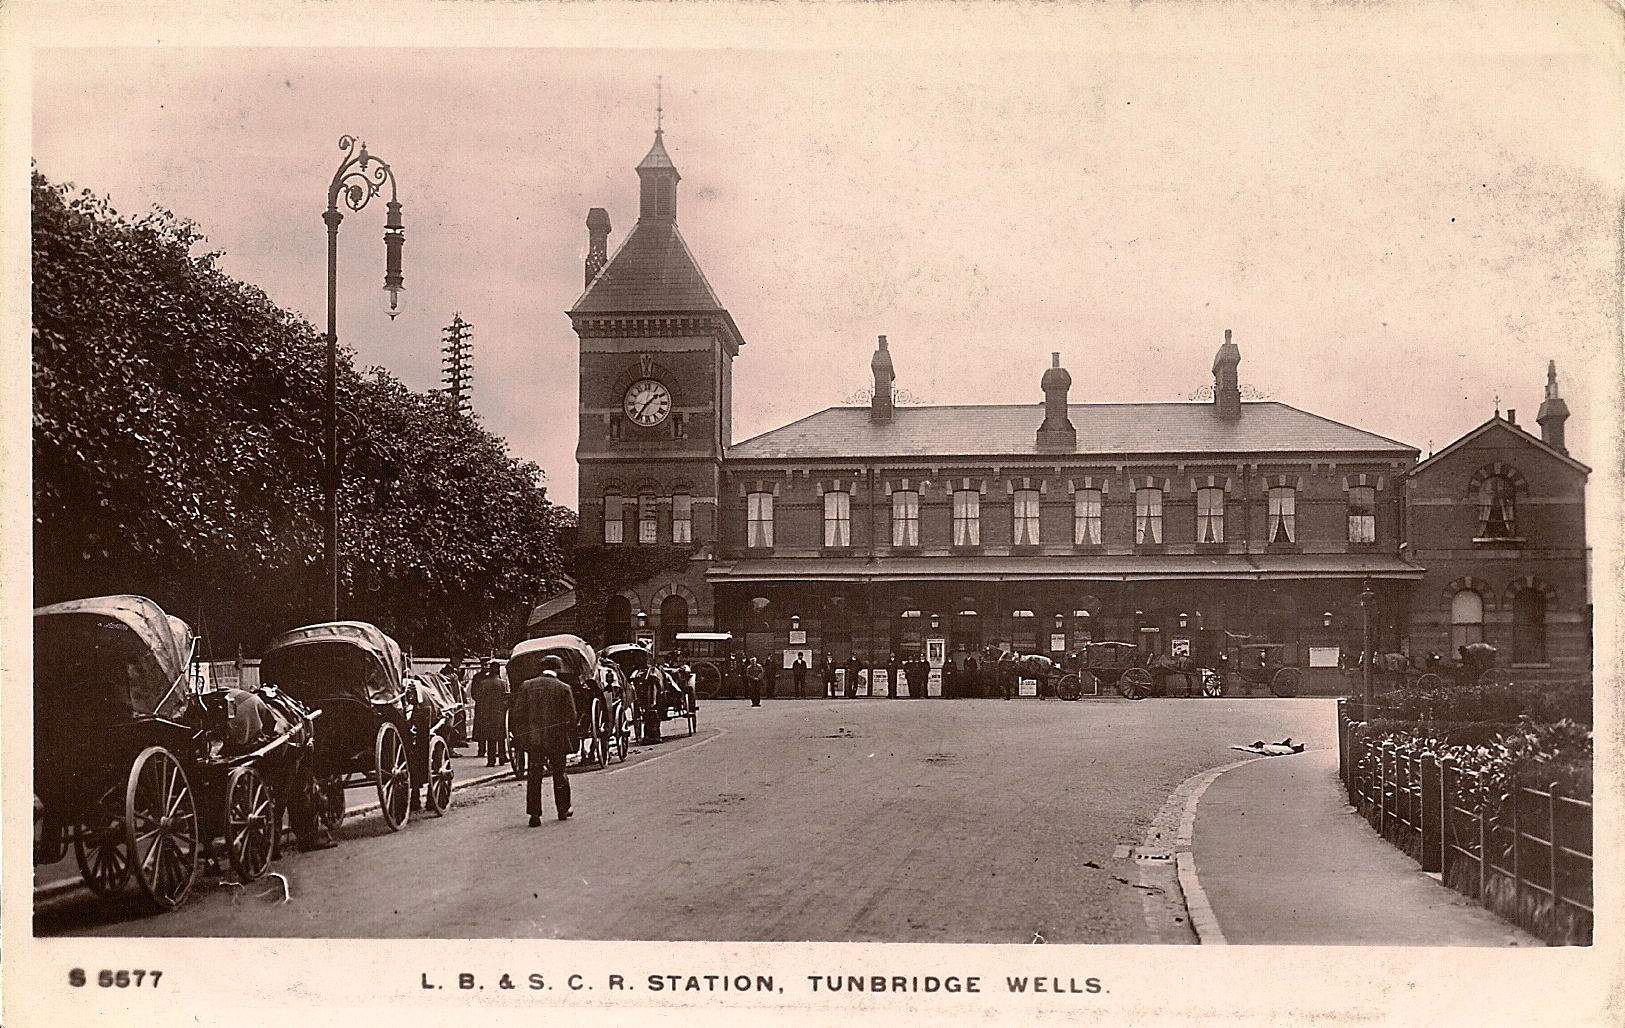
\includegraphics[width=0.6\textwidth]{./figures/tunbridgeWells.jpg}}
		\end{figure}
		
	\end{frame}

	\begin{frame}
		\frametitle{Course outline}
		
		\begin{itemize}
			\item 9am-10.30am: follow along lecture and problems
			\item 10.30am-10.45am: refreshments break
			\item 10.45am-midday: follow along lecture and problems
		\end{itemize}
		
		\vspace{0.5cm}
		
		Note: problems will involve both pen and paper type questions \textit{and} those using R.
		
		Levels: each problem set will have at least one \textit{advanced} question.
		
		Time: if you don't finish the questions in time, don't worry. There are answers to these here: 
		
	\end{frame}

	\begin{frame}
		\frametitle{Resources}
		
		\begin{itemize}
			\item Introduction to probability, Blitzstein and Hwang. Open source book available here: \url{https://projects.iq.harvard.edu/stat110/home}
			\item Seeing theory, Kunin et al. A beautiful online resource that has lots of creative ways to think about probability. \url{https://seeing-theory.brown.edu/}
		\end{itemize}
		
	\end{frame}

	\begin{frame}
		\frametitle{Outline}
		\tableofcontents
	\end{frame}

	\section{What is probability and why do we need it?}
	\frame{\tableofcontents[currentsection]}
	
	\begin{frame}
		\frametitle{What is probability?}
		\epigraph{Mathematics is the logic of certainty; probability [theory] is the [mathematical] logic of uncertainty}{Bitzstein and Hwang, 2019}
		
	\end{frame}

	\begin{frame}
		\frametitle{Why do we need probability theory?}
		
		Life and science are full of unknown things. We say these things are \textit{uncertain}.
		
		Faced with these, we can give up; \textit{Probability theory} gives us a way to make assumptions about uncertain phenomena which allows us to make progress with understanding without having to know everything.
		
		\epigraph{There are known knowns. These are things we know that we know. There are known unknowns. That is to say, there are things that we know we don't know. But there are also unknown unknowns. There are things we don't know we don't know.}{Donald Rumsfeld, 2002}
		
	\end{frame}
	
	\begin{frame}
		\frametitle{Who uses probability?}
		It is used in:
		
		\begin{itemize}
			\item Statistics: probability is the foundational language of it
			\item Biology: e.g. inheritance of genes
			\item Meteorology: e.g. weather forecasts are generated using probabilities
			\item Epidemiology: e.g. analysing randomised clinical trials and fitting models to epidemiological data
			\item Physics: our current best explanation of the universe at small scales (quantum theory) is based on probability
		\end{itemize}
		
		
	\end{frame}

	\begin{frame}
		\frametitle{The difficulties of probability}
		
		If we rely on our intuitions, we can easily get things wrong when dealing with uncertainty.
		
		\vspace{0.5cm}
		
		 So, we need careful mathematical analysis.
		 
		 \vspace{0.5cm}
		
		Fortunately, \textit{simulation} using R / Python / etc. can also really help us to understand.
		
	\end{frame}

	\section{Probability and counting}
	\frame{\tableofcontents[currentsection]}
	
	\begin{frame}
		\frametitle{Blitzstein and Hwang's Pebble World}
		
		As an example, consider reaching into a bag to pull out one of nine pebbles: we call this \textit{pebble world}.
		
		\begin{figure}[ht]
			\centerline{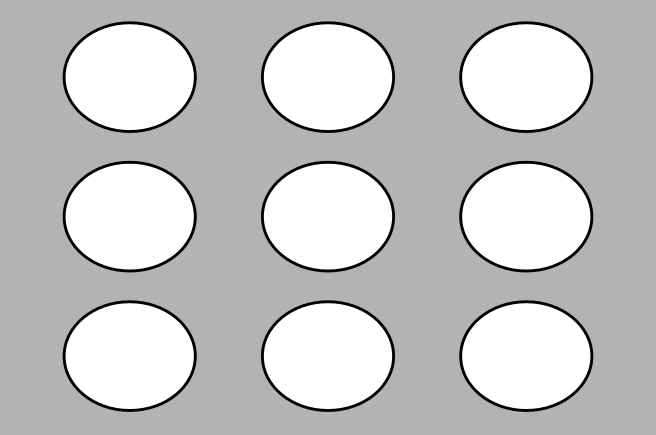
\includegraphics[width=0.6\textwidth]{./figures/pebble_world_base.png}}
		\end{figure}
		
	\end{frame}


	\begin{frame}
		\frametitle{Outcomes}
		
		An \textit{outcome} is a possible result of some activity. Here pulling one particular pebble out of the bag would be an outcome.
		
		\begin{figure}[ht]
			\centerline{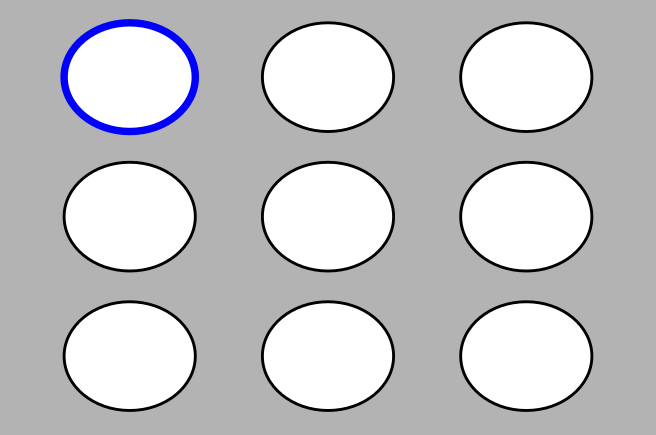
\includegraphics[width=0.6\textwidth]{./figures/pebble_world_single.png}}
		\end{figure}
		
	\end{frame}

	\begin{frame}
		\frametitle{Sample spaces}
		
		The \textit{sample space}, $S$, is the \textit{set} of all possible outcomes of an experiment. Here, it is the set of all pebbles.
		
		\begin{figure}[ht]
			\centerline{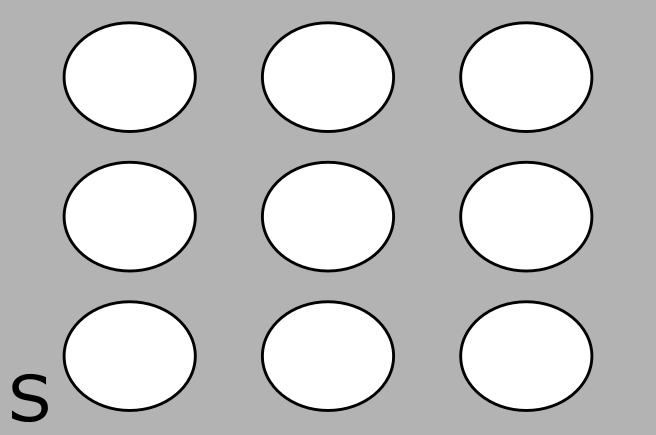
\includegraphics[width=0.6\textwidth]{./figures/pebble_world_sample_space.png}}
		\end{figure}
		
	\end{frame}

	\begin{frame}
		\frametitle{Events}
		
		An \textit{event} is a \textit{set} of possible outcomes. For example, below event $A$ corresponds to selecting one of five pebbles; event $B$ to selecting one of two.
		
		As we can see, two or more events can happen at once.
		
		\begin{figure}[ht]
			\centerline{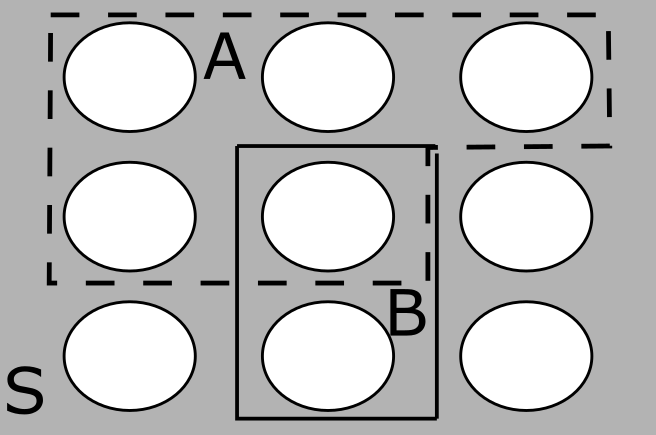
\includegraphics[width=0.6\textwidth]{./figures/pebble_world.png}}
		\end{figure}
		
	\end{frame}


	\begin{frame}
		\frametitle{Probabilities of events}
		
		What do we mean by the probability of $A$ occurring? We write this as: $\mathbb{P}(A)$.
		
		\begin{figure}[ht]
			\centerline{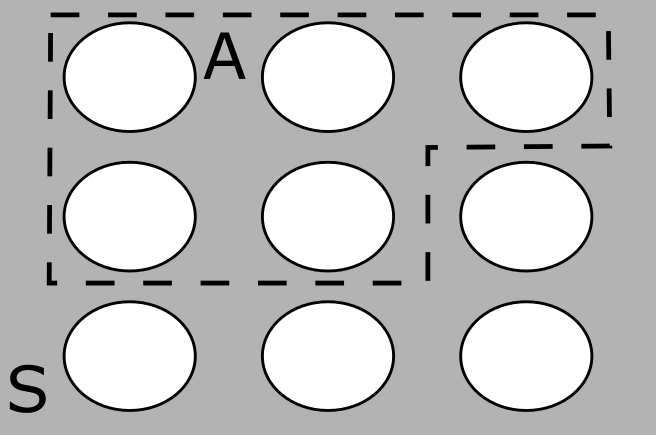
\includegraphics[width=0.6\textwidth]{./figures/pebble_world_proba.png}}
		\end{figure}
		
	\end{frame}

	\begin{frame}
		\frametitle{Probabilities from counting}
		
		If all pebbles equally likely to be drawn:
		
		 \begin{equation}
		 	\mathbb{P}(A) = \frac{\text{number of pebbles in } A}{\text{number of pebbles in } S} = \frac{5}{9}
		 \end{equation}
	 
	 \begin{figure}[ht]
	 	\centerline{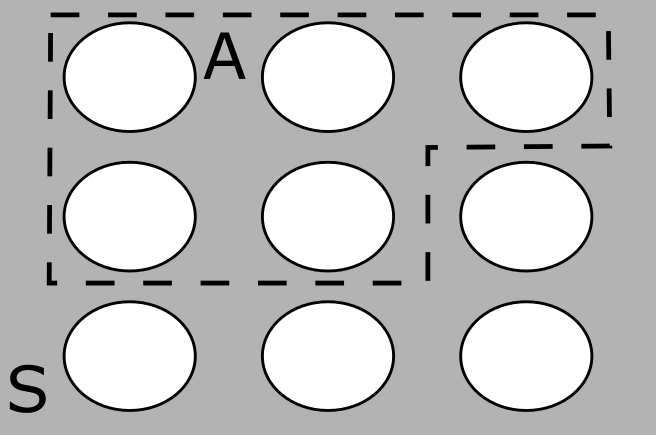
\includegraphics[width=0.6\textwidth]{./figures/pebble_world_proba.png}}
	 \end{figure}
		
	\end{frame}

	\begin{frame}
		\frametitle{Probability of an event in $S$}
		
		Consider the probability that some event in $S$ occurs:
		
		\begin{equation}
			\mathbb{P}(S) = \frac{\text{number of pebbles in } S}{\text{number of pebbles in } S} = \frac{9}{9} = 1
		\end{equation}
		
		\begin{figure}[ht]
			\centerline{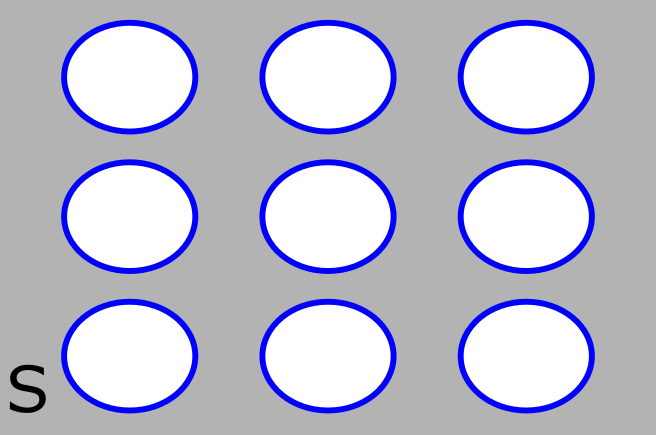
\includegraphics[width=0.6\textwidth]{./figures/pebble_world_probs.png}}
		\end{figure}
		
	\end{frame}

	\begin{frame}
		What about the probability that no event in $S$ occurs?
		
		\begin{equation}
			\mathbb{P}(\text{not }S) = \frac{0}{9} = 0
		\end{equation}
		
		\begin{figure}[ht]
			\centerline{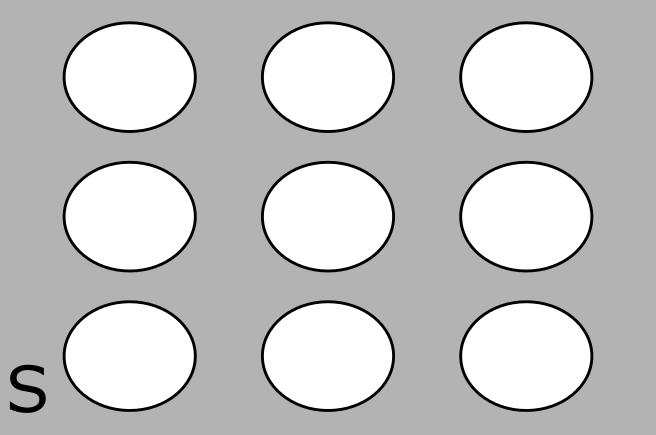
\includegraphics[width=0.6\textwidth]{./figures/pebble_world_probnots.png}}
		\end{figure}
		
	\end{frame}

	\begin{frame}
		\frametitle{Defining probability}
		
		A probability of an event must be bounded between 0 and 1\footnote{Note: ``impossible'' isn't 100\% accurate here but you can start out by thinking of probabilities this way.}.
		
		\begin{figure}[ht]
			\centerline{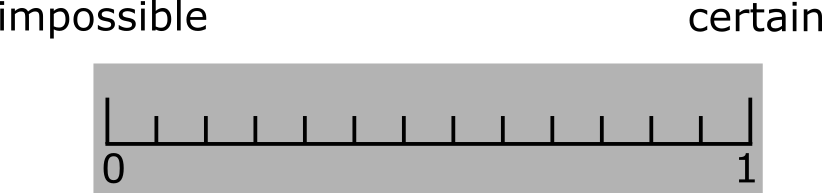
\includegraphics[width=0.8\textwidth]{./figures/probability.png}}
		\end{figure}
		
	\end{frame}

	\begin{frame}
		\frametitle{Interpreting probabilities}
		
		There are many schools of thought for what probabilities mean. Two common ones are:
		
		\begin{itemize}
			\item \textit{Frequentist}. Think of probabilities as frequencies that would be obtained under many (actually infinite) repetitions of an experiment. E.g. flipping a coin a large number of times and using fraction of heads as $\mathbb{P}(H)$.
			\item \textit{Bayesian}. Suppose probabilities reflect an underlying subjective belief about the chance of events occurring.
		\end{itemize}
		
	\end{frame}

		\begin{frame}
		\frametitle{An event not occurring}
		We can also determine the probability that $A$ does not occur:
		
		\begin{equation}
			\mathbb{P}(\text{not } A) = \frac{\text{number of pebbles not in } A}{\text{number of pebbles in } S} = \frac{4}{9}
		\end{equation}
		
		\begin{figure}[ht]
			\centerline{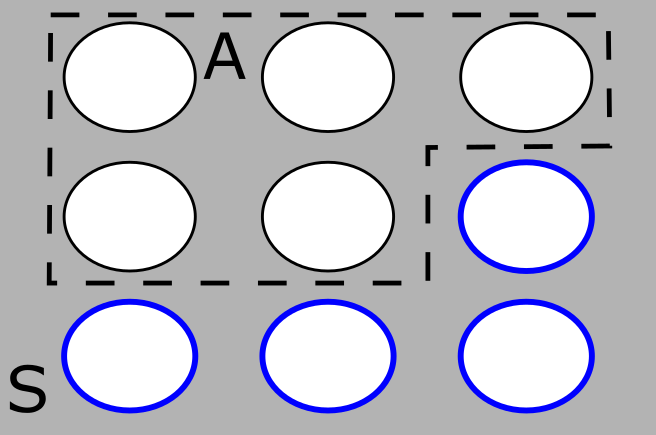
\includegraphics[width=0.6\textwidth]{./figures/pebble_world_probnota.png}}
		\end{figure}
		
	\end{frame}

	\begin{frame}
		\frametitle{Question}
		
		\Large Can anyone think of an alternative way of determining the probability that $A$ does not occur?
		
	\end{frame}

	\begin{frame}
		\frametitle{Question}
		
		\Large Can anyone think of an alternative way of determining the probability that $A$ does not occur?
		
		\begin{equation}
			\mathbb{P}(\text{not } A) = \mathbb{P}(S) - \mathbb{P}(A) = 1 - \mathbb{P}(A) = 1 - \frac{5}{9}
		\end{equation}
		
	\end{frame}

	\begin{frame}
		\frametitle{Combinations of events: intersection}
		
		We can determine the probability of $A$ \textit{and} $B$ occurring by determining the overlap between these two events:
		
		\begin{equation}
			\mathbb{P}(A \cap  B) = \mathbb{P}(A, B) = \frac{\text{number of pebbles in both } A \text{ and } B}{\text{number of pebbles in } S} = \frac{1}{9}
		\end{equation}
		
		\begin{figure}[ht]
			\centerline{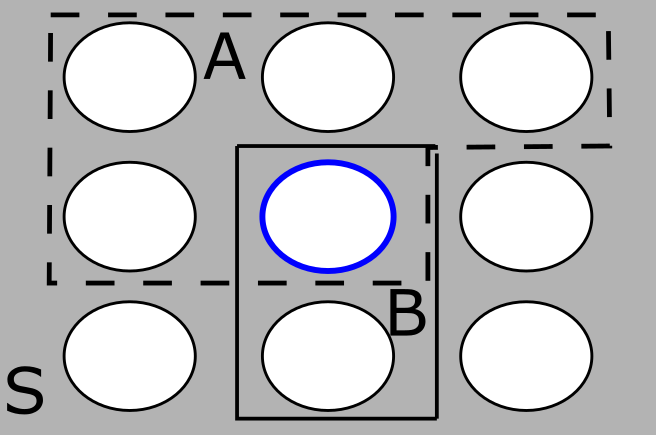
\includegraphics[width=0.6\textwidth]{./figures/pebble_world_and.png}}
		\end{figure}
		
	\end{frame}

	\begin{frame}
		\frametitle{Combinations of events: union}
		
		We can determine the probability of $A$ \textit{and/or} $B$ occurring by:
		
		\begin{equation}
			\mathbb{P}(A \cup B) = \frac{\text{number of pebbles in either } A \text{ or } B \text{ or both}}{\text{number of pebbles in } S} = \frac{6}{9}
		\end{equation}
	
	\begin{figure}[ht]
		\centerline{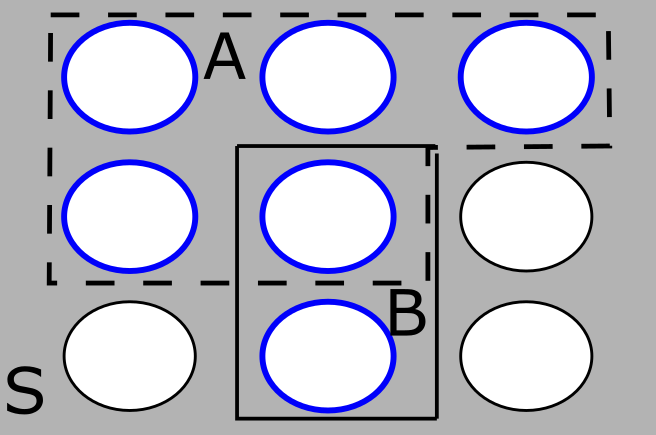
\includegraphics[width=0.6\textwidth]{./figures/pebble_world_or.png}}
	\end{figure}
		
	\end{frame}

	\begin{frame}
		\frametitle{Question}
		
		\Large Can anyone think of an alternative way of determining the probability of the union of $A$ and $B$?
		
	\end{frame}

	\begin{frame}
		\frametitle{Question}
		
		\Large Can anyone think of an alternative way of determining the probability of the union of $A$ and $B$?
		
		\begin{align}
			\mathbb{P}(A \cup B) &= \mathbb{P}(A) + \mathbb{P}(B) - \mathbb{P}(A \cap B)\\
			&= \frac{5}{9} + \frac{2}{9} - \frac{1}{9} = \frac{6}{9}
		\end{align}
		
		
	\end{frame}
	
	
	\begin{frame}
		\Large Questions?
	\end{frame}
	
	
	\begin{frame}
		\frametitle{Problems: dice}
		
		\begin{figure}[ht]
			\centerline{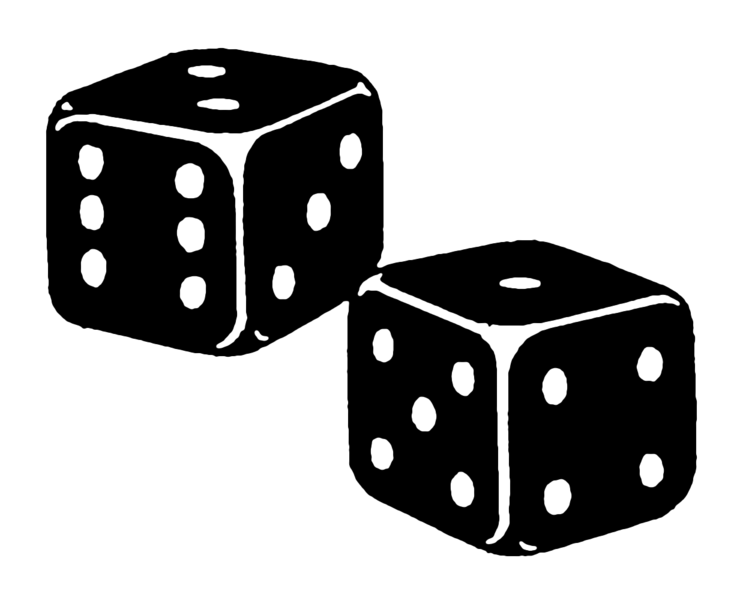
\includegraphics[width=0.2\textwidth]{./figures/dice.png}}
		\end{figure}
	
	Consider a six-sided die with numbers 1-6 on each face that is thrown once.
		
		\begin{enumerate}
			\item What's the probability that a six is thrown?
			\item What's the probability that an even number is thrown?
			\item Suppose two dice are thrown, what's the probability that the their sum adds up to 11 or less?
			\item \textit{Advanced}: if six dice are thrown, what's the probability that one of each of the numbers is obtained?
		\end{enumerate}
		
	\end{frame}


	\begin{frame}
		\frametitle{Example: a random sweet}
		
		Suppose you visit a sweet shop. The shop produces both ice cream and cake. It also offers three sauces: strawberry, vanilla and chocolate.
		
		\vspace{0.5cm}
		
		Unlike most shops, you don't get a choice. The way the shopkeeper allocates food is they randomly choose either a ice cream or cake (selecting either with equal probability). They then randomly select a sauce from the three available (again with equal probability of each).
		
		\vspace{0.5cm}
		
		Suppose you like anything with chocolate sauce. What's the probability that you obtain this?
		
	\end{frame}

	\begin{frame}
		\frametitle{A naive way to count}
		
		How many outcomes are there? Cake with strawberry, cake with vanilla, cake with chocolate, ice cream with strawberry, ice cream with vanilla, ice cream with chocolate.  So there are \textit{six} outcomes.
		
		\vspace{0.5cm}
		
		How many of these have chocolate sauce: two.
		
		\vspace{0.5cm}
		
		\begin{equation}
			\mathbb{P}(\text{chocolate}) = \frac{2}{6}
		\end{equation}
		
	\end{frame}


	\begin{frame}
		\frametitle{A sweet tree: making counting easier}
		
		\begin{figure}[ht]
			\centerline{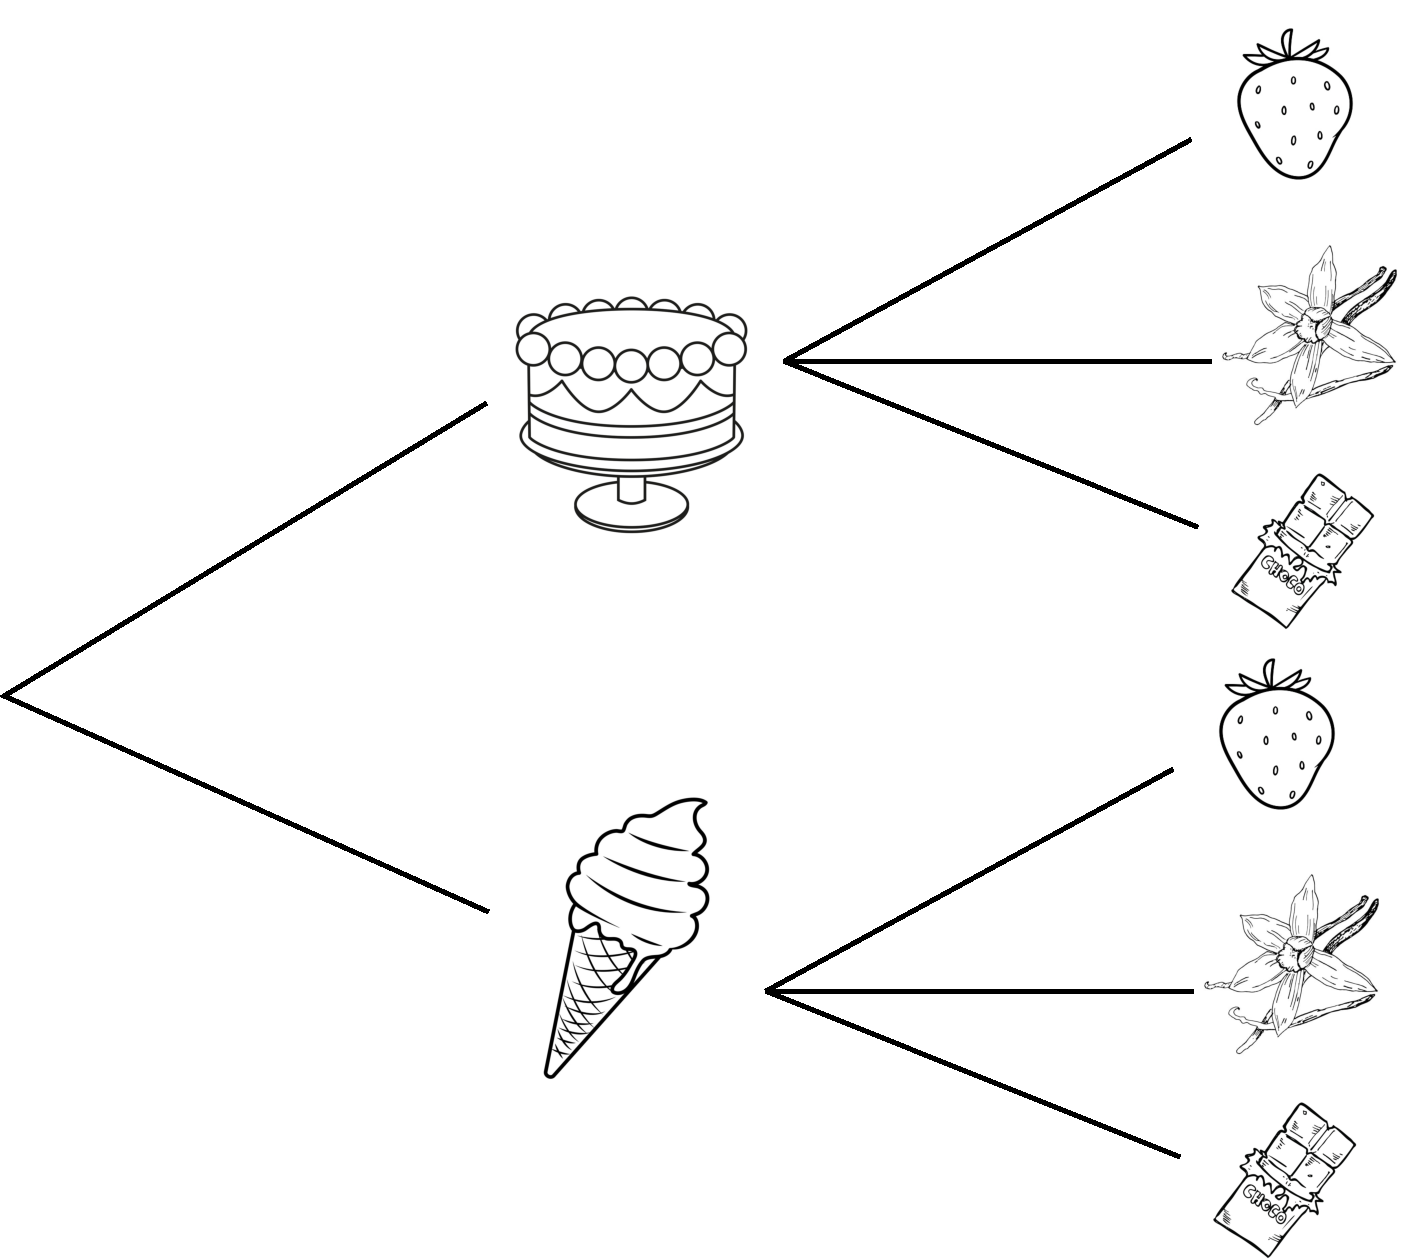
\includegraphics[width=0.7\textwidth]{./figures/tree.pdf}}
		\end{figure}
		
	\end{frame}

	\begin{frame}
		\frametitle{Using trees to determine probabilities}
		
		\begin{figure}[ht]
			\centerline{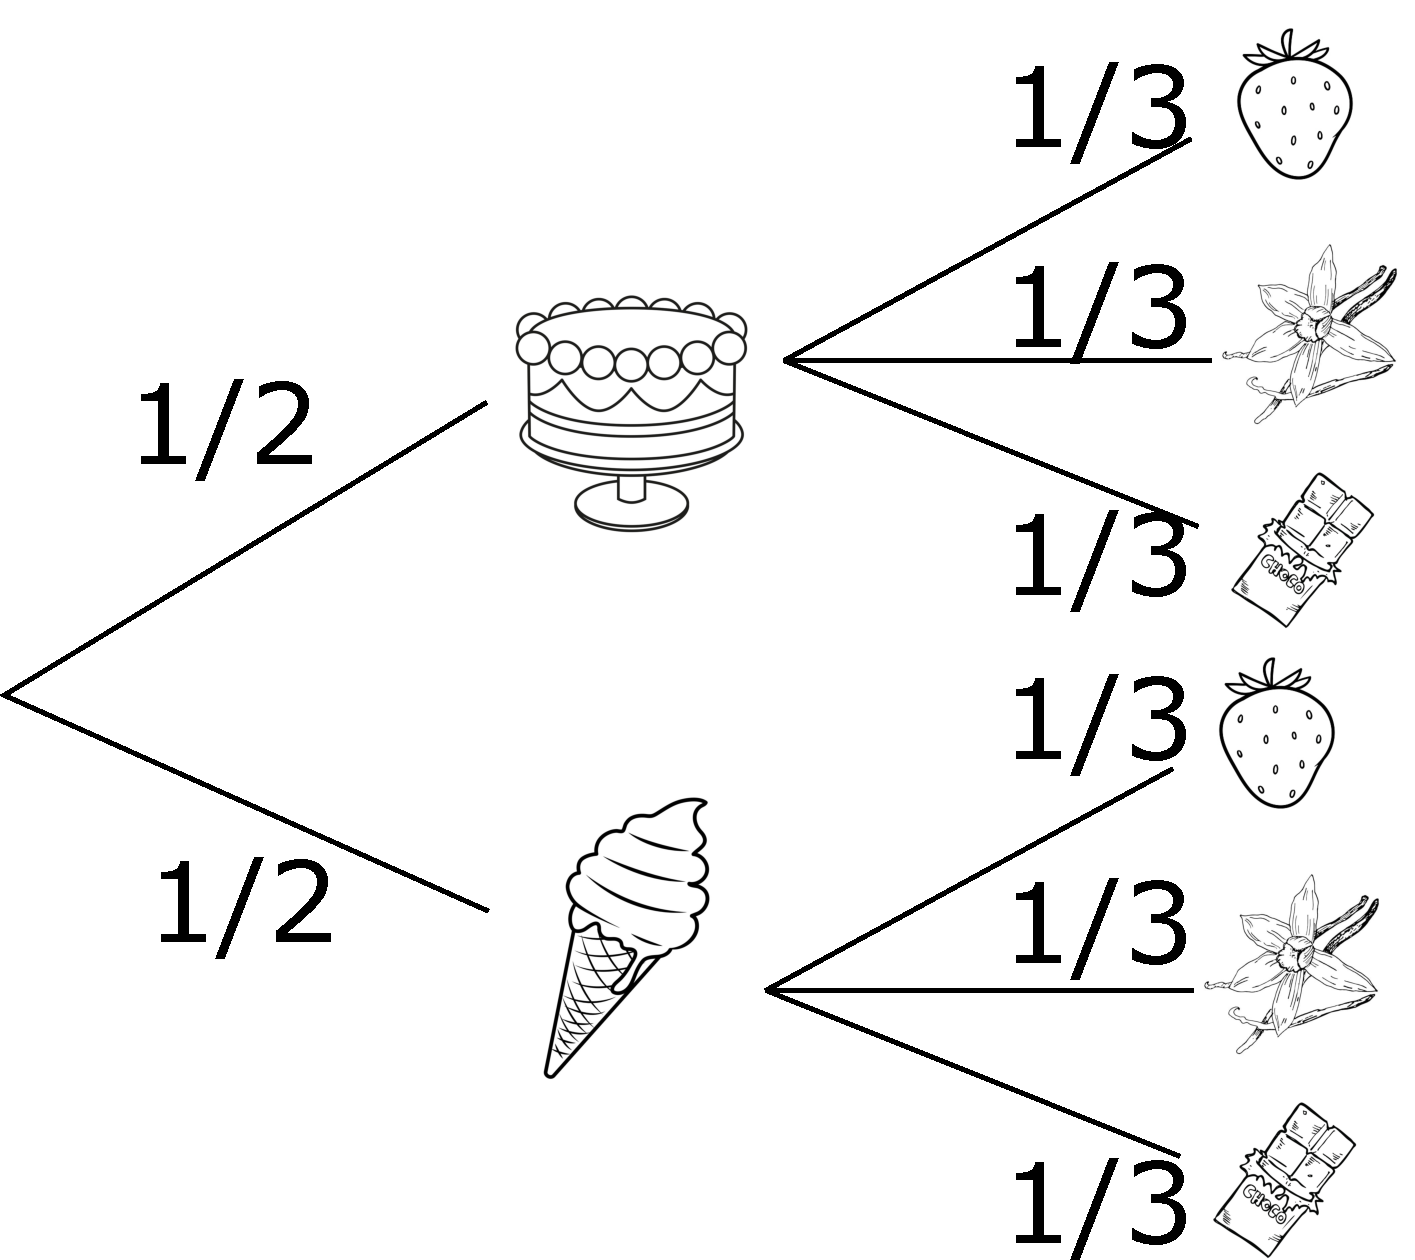
\includegraphics[width=0.7\textwidth]{./figures/tree-prob.pdf}}
		\end{figure}
		
	\end{frame}

	\begin{frame}
		\frametitle{What's the probability of cake with chocolate sauce?}
		
		\begin{figure}[ht]
			\centerline{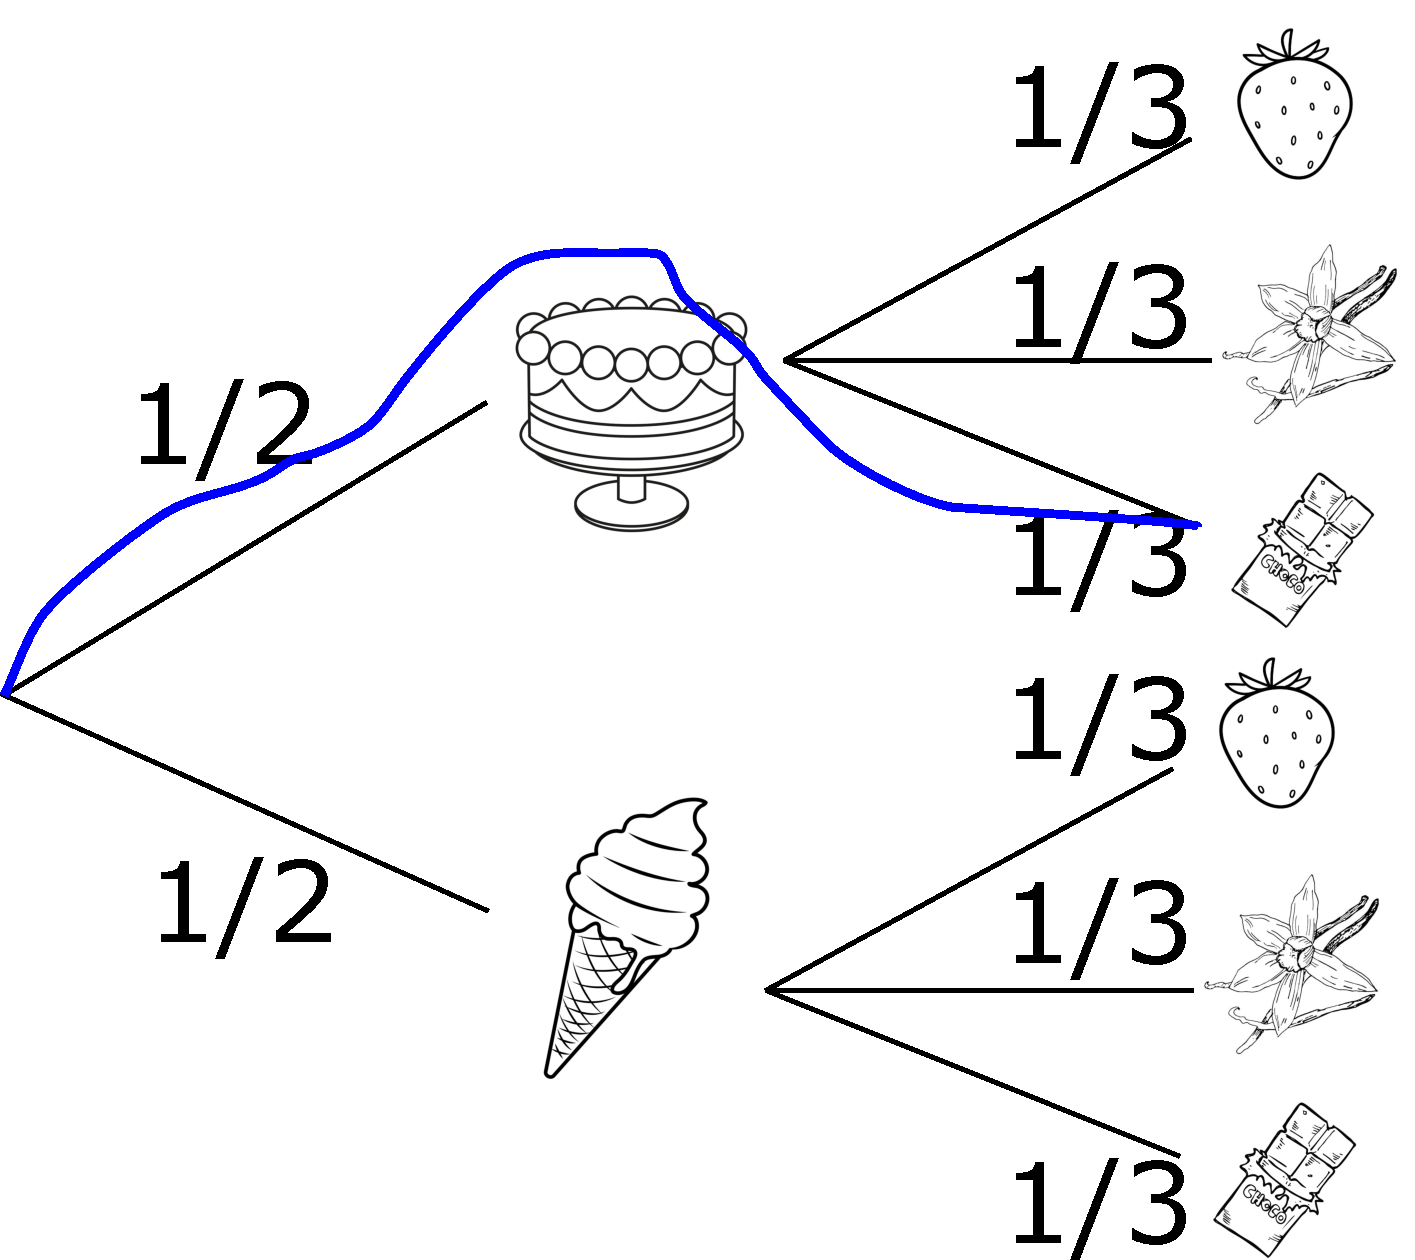
\includegraphics[width=0.4\textwidth]{./figures/tree-prob-choc-cake.pdf}}
		\end{figure}
	
	To obtain this probability, we take the probabilities obtained along the path and multiply:
	
	\begin{equation}
		\mathbb{P}(\text{chocolate cake}) = \frac{1}{2} \times \frac{1}{3} = \frac{1}{6}
	\end{equation}


	This is equivalent to counting possibilities (if all choices equally likely).
	
	\end{frame}

	\begin{frame}
		\frametitle{Chocolate probability}
		
		\begin{figure}[ht]
			\centerline{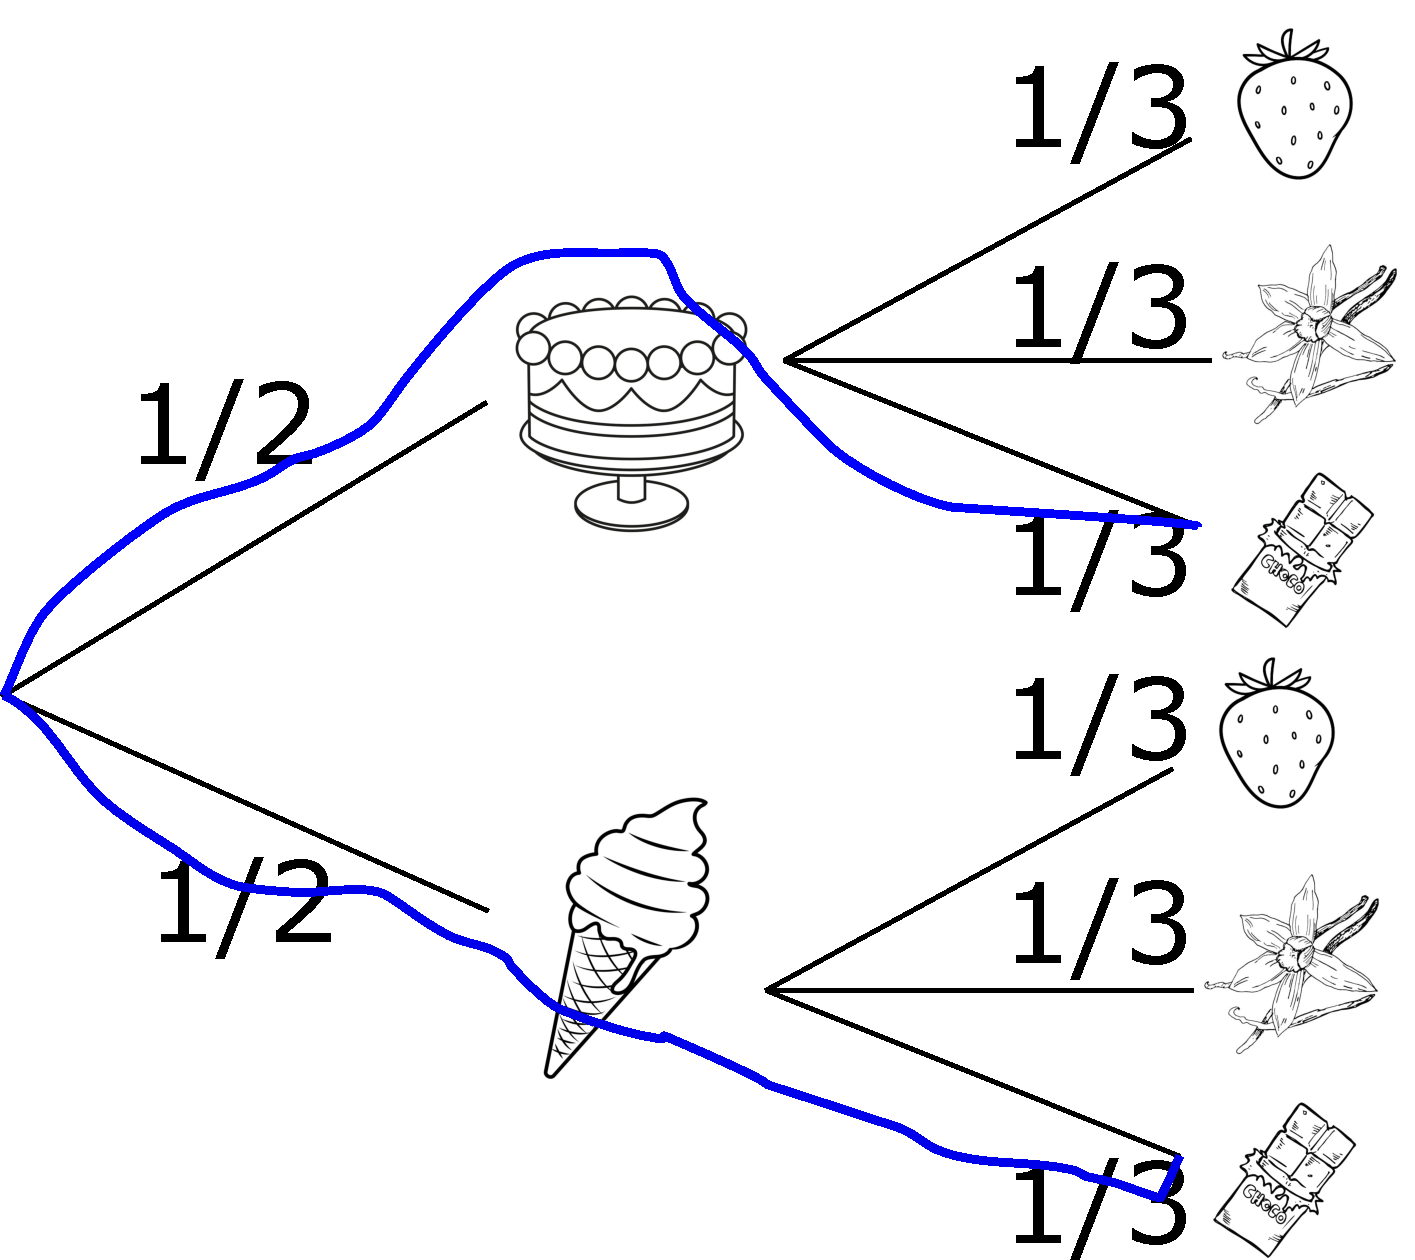
\includegraphics[width=0.4\textwidth]{./figures/tree-prob-choc.pdf}}
		\end{figure}
	
	Sum up probabilities:
	
	\begin{equation}
		\mathbb{P}(\text{chocolate}) = \frac{1}{2} \times \frac{1}{3} +  \frac{1}{2} \times \frac{1}{3} = \frac{2}{6}
	\end{equation}
	
	\end{frame}

	\begin{frame}
		\frametitle{A particular shopkeeper}
		Now suppose we visit another shop. Here, the shopkeeper allocates cake or ice cream as before (i.e. with equal probability). The differ in terms of how they offer sauces:
		
		\vspace{0.5cm}
		
		If a cake is chosen, they randomly select sauces: vanilla with probability $1/2$, chocolate with probability $1/3$ and strawberry with probability $1/6$.
		
		\vspace{0.5cm}
		
		If an ice cream is chosen, they randomly select sauces: vanilla with probability $1/6$, chocolate with probability $1/2$ and strawberry with probability $1/3$.
		
		\vspace{0.5cm}
		
		Now what is the probability an item with chocolate sauce is obtained?
		
	\end{frame}

	\begin{frame}
		\frametitle{The problem with counting}
		
		
		
	\end{frame}


	\section{Conditional probability}
	\frame{\tableofcontents[currentsection]}
	
	\begin{frame}
		\frametitle{What is conditioning?}
		
		When we receive new information, we want to take it into account to make better predictions.
		
		\vspace{0.5cm}
		
		Effectively, learning something about the world (typically) helps us to reduce our own uncertainty.
		
		\vspace{0.5cm}
		
		\textit{Conditioning} is how this is handled in statistics.
		
	\end{frame}

	\begin{frame}
		Independence
	\end{frame}
	

	\section{Random variables and probability distributions}


	\section{Joint distributions}
	\frame{\tableofcontents[currentsection]}

	\section{Marginal and conditional probability}
	\frame{\tableofcontents[currentsection]}
	
	\section{Bayes' rule}
	\frame{\tableofcontents[currentsection]}
	
	Use breast cancer example.
	
	\section{Continuous probability distributions}
	\frame{\tableofcontents[currentsection]}
	
\end{document} 